\subsection{Merkle Trees}\label{sec:hash_functions:merkle_tree}

A \textbf{Merkle tree} is a cryptographic data structure used to efficiently verify the integrity of large datasets. Concretely, a Merkle tree is a binary tree (\Cref{figure:merkle_tree}) where each \textbf{leaf node} contains the digest of a \textbf{data block}, and each non-leaf node (or \textbf{intermediate node}) contains the digest of its two child nodes. The \textit{root node}, known as the \textbf{Merkle root}, serves as a unique fingerprint of the entire dataset. For instance, in \Cref{figure:merkle_tree} H1 is the digest of the data block D1, H34 is the digest of the concatenation of H3 and H4, and H1234 (the Merkle root) is the digest of the concatenation of H12 and H34. Any modification to any data block causes the Merkle root to change.

\begin{figure}[t!]
	\begin{center}
		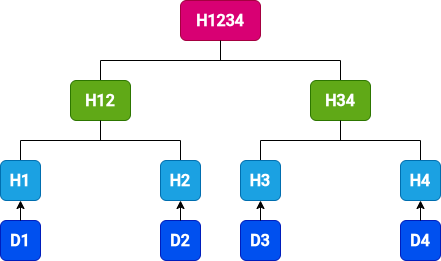
\includegraphics[width=0.75\linewidth]{resources/img/merkle_tree.png}
		\caption{A simple Merkle tree}
		\label{figure:merkle_tree}
	\end{center}
\end{figure}

Merkle trees are widely employed in distributed systems --- e.g., version control systems such as Git, blockchains (\Cref{sec:popular_applications:blockchain}), distributed peer-to-peer networks such as BitTorrent, and distributed databases such as Cassandra --- to ensure data integrity with minimal effort.
